%\chapter{State of the art} 
\label{chapter:stateofart} 

\section{Migraine disease}

Migraine is a very common chronic disorder that affects over 16\% and 8\% of world women and men, respectively. It has two major subtypes: migraine with and without aura. Both are characterized by headache and specific associated symptoms, whereas the former also includes neurological symptoms that precede the headache. Some patients also experience a premonitory phase, occurring hours or days before the headache, a postdrome or resolution and a recovery phase. Premonitory and resolution symptoms include hyper or hipoactivity, depression, cravings for particular foods, repetitive yawning, fatigue and neck stiffness and/or pain.


The present diagnosis of the migraine illness is usually performed through the symptoms and the headache description reported by the patient, comparing them with the criteria of the \emph{The International Classification of Headache Disorders} \cite{pmid23771276}. Its current management and treatment are heterogeneous, normally pharmacological, and depends on the symptoms, the type of migraine, and the chronification level of the disease \cite{diener2012chronic, hershey2010current, silberstein2012safety, guglielmo2013possible, lopes2012concepts}. Their accuracy is determined by the moment when the patients take their medication. This is usually so late that the headache arrives and the patient suffers the migraine disturbances equally.


Because there is a significant percentage of migraineurs that are not satisfied with that lack of effect of the treatments \cite{smelt2014patients,HEAD:HEAD1867}, in order to continue understanding the triggers and symptoms of migraine disease, several studies have been performed through the years: electrocardiogram (ECG) \cite{melek2007autonomic, aygun2003electrocardiographic}, heart rate \cite{pmid23853566, pmid19925627}, skin temperature \cite{zaproudina2013acral, ordas2013increase}, blood pressure \cite{pietrini2005hypertension, pmid19925627}, electroencephalogram (EEG)  \cite{bjork2011initiates, walker2011qeeg}, and cortical spreading depression  \cite{charles2013cortical} among others. Mostly are related to physiological human variables, but also some meteorological researches have been carried out \cite{bolay2011does, friedman2009migraine, prince2004effect}. However, the causes of migraine attacks are still unknown and the conclusions are sometimes conflicting.


\section{e-Health}

e-Health is a term used to describe the application of Information and Communication Technologies (ICT) to the Health field. e-Health technologies are very varied in terms of objectives, people involved and technology. They are divided into three different areas \cite{black2011impact}: storing, managing, and transmission of data; clinical decision support; and facilitating care from a distance. Within these categories, we found a wide list of e-Health components that are currently being developed: electronic clinical history \cite{schiff2010can}, telemedicine \cite{anker2011telemedicine}, standardization and interoperability \cite{kanter2012importance,aragues2011trends}, online health information websites \cite{van2010definition}, interactive electronic health records \cite{archer2011personal}, health decision support programs \cite{romano2011electronic}, the mobile health (m-Health) \cite{kay2011mhealth}, etc.

Among these components, the m-Health has increased its world presence due to the advances in mobile and wearability technologies (see \figref{e2m_health} extracted from \cite{pawar2012framework}). Since m-Health tools enable monitoring the type, quantity, and quality of everyday activities of users, it is becoming an almost infinite clinical, sportive, and research source of information. It allows to improve daily care, design more clinically meaningful randomized trials of interventions, and establish cost-effective, evidence-based practices \cite{dobkin2011promise}.

This wide extension of the m-Health is obvious in the variety of companies that perform some  activity on the Personal Health System market --for instance, Nintendo, Microsoft, Google, Medtronic, Intel, Nike, Cambridge Silicon Radio Orange or Bayer \cite{baum2013market}--  and also in its heterogeneous current applications --physical activity assessment \cite{wuttidittachotti2014mhealth, o2013current}, cardiac rehabilitation \cite{pfaeffli2012mhealth}, sports \cite{verhagen2013peek} and remote diagnostics and consultation \cite{godoy2013virtual}. The common denominator in all these applications seem to be the Wireless Body Sensor Networks.

\begin{figure}[!ht]
\centering
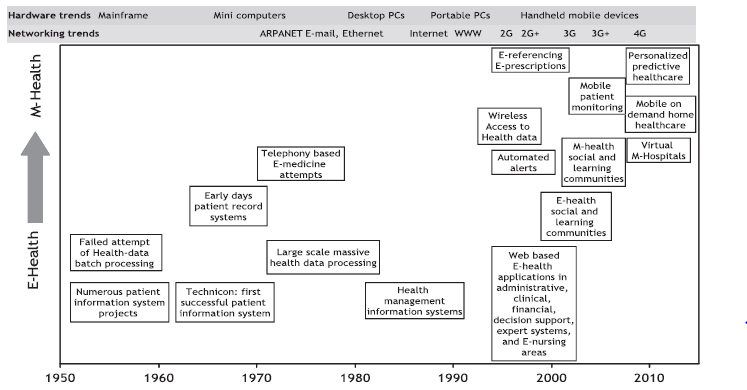
\includegraphics[width=\textwidth]{images/ehealth_evol.png}
\caption{Evolution over the time from the e-Health to the m-Health}
\label{fig:e2m_health}
\end{figure}

Wireless Sensor Network (WSN) is an emerging technology area based on the utilization of wireless gadgets to build a complete ICT-based wireless monitoring system. It consists of many nodes that can communicate with each other with routing responsibilities. Each node is equipped with a sensing unit, a memory, a microcontroller, a wireless communication interface and a power source.


The growing interest in the use of WSNs has been driven by the large number of emerging applications, such as home and industrial automation \cite{gomez2010wireless,akerberg2011future}, process monitoring \cite{zapater2012ubiquitous, khanna2012machine} and healthcare applications \cite{journals/jst/AbidoyeAAAN11, ko2010wireless, pawar2012framework}. They enable dense and flexible deployments at low cost.


One of the most promising uses of WSNs is the healthcare monitoring. It requires special wearable sensors placed on the  body surface. This peculiarity gives its name to the Wireless Body Sensor Network, in which spatially distributed sensors, each equipped with a radio transceiver --normally, Bluetooth or ZigBee ones \cite{chen2013review}--, cooperate with each other to monitor physiological or environmental human conditions. This kind of networks are usually integrated into a broader multitier telemedicine system \cite{Otto:2005:SAW:2010498.2010502, journals/jst/AbidoyeAAAN11, chen2013review, jovanov2011body, jovanov2009system}.


The amount of different types of measures currently provided by WBSNs is extensive:  electroencephalogram \cite{dilmaghani2011wireless}, stress \cite{jovanov2003stress}, emotions \cite{nasoz2004emotion}, blood pressure \cite{espina2006wireless} and accelerometry \cite{chung2008wireless} among others.



\section{Algorithms for wearable sensors in health monitoring systems}

As we have mentioned before, nowadays we are witnessing an increase in the development of wearable sensors for health monitoring systems. An important aspect of study in such systems is how the data gathered -in particular continuous time series measurements- are treated and processed. 

The integration and interpretation of the sensor signals usually pursue anomalies detection, prediction or decision making \cite{banaee2013data}. Therefore, the idea is to extract relevant medical information from large physiological data sets. Known in a wider context as \emph{data mining}, this intention normally becomes a computational process that involves artificial intelligence, machine learning, statistics and database systems.

The set of available methods and algorithms of data mining is very varied.The most common ones and their main characteristics and applications are listed below:

\begin{description}
	
	\item{\textbf{Support Vector Machines}\hfill \\
	The Support vector machines (SVM) technique is one of the main learning methods applied in classification and regression. Being primarily designed for two-class problems, the method derives some selected features from well known data and finds the optimal hyperplane -a linear classifier- to separate the unseen information into two classes in order to make a decision model \cite{cortes1995support}. 

	It is widely use for anomaly detection and decision making because of its ability to distinguish (non)healthy patterns. For instance, SVMs have been used to find out arrhythmia in ECG signals \cite{hu2008robust} and seizure episodes \cite{lee2012low}. 

	However, SVM is not an appropriate method to integrate domain knowledge and cannot be applied to find the unexpected information from unlabeled data.}

	\item {\textbf{Hidden Markov Models}\hfill \\
	A Markov Model is a stochastic process where it is assumed that the future states of a changing system depend only on the current one. In the Hidden Markov Models (HMM), some of these states are hidden from an observer in the sense that an observer cannot directly determine which state the system is in at any given point in time. However, a number of observable parameters dependent on the current state of the system are visible. Based on the visibility of this dependance, the occurrence probability of each state can be compute \cite{quwaider2008body}.

	HMM models are especially applied to temporal pattern recognition because of its ability for modeling sequential data. They have been used, for example, to detect abnormal values in blood glucose level \cite{zhu2011automatic} and perform a probabilistic segmentation for populating medical time series databases \cite{woodbridge2011salient}.}

	\item {\textbf{Artificial Neural Networks}\hfill \\
	Artificial Neural Networks (ANN) try to emulate the way in which biological neurons integrate and process the information of the brain. The basis of this technique lies on how the combination of the simple behaviour of each artificial neuron can result in a network with a much more complex performance. Thus, by applying different weights and non-linear functions to the input signals, the ANNs are able to model complex relationships where the correlation among the input parameters is not easily detectable \cite{al2011artificial}.

	ANNs are widely used for complex classification and prediction tasks in the medical domain. For instance, they have been used to assess the clinical quality of the pulses in PPG \cite{li2012dynamic} or to recognize heart rate variability patterns using ECG and accelerometer sensors \cite{vu2010online}. ANNs have also been proposed to predict blood glucose levels \cite{chatterjee2013persuasive}.}

	\item {\textbf{Decision Trees}\hfill \\
	Based on recursive data segmentation, decision trees provides an efficient representation of rule classification. During the process, the
	features of the input data are selected by descending order of robustness. That way, data is splitted by creating a tree-like model.

	This method has been proposed for the discrimination of emotional physiological signals evoked \cite{frantzidis2010classification}, for on-body heat stress risk prediction \cite{gaura2013leveraging}, and many other applications.

	Decision trees are simple and easy to implement.However, its efficiency worsen with the number of features to deal with, so these models are not usually applied to big and complex data.
	}

\end{description}

Other techniques widely used in diagnosis, prediction and decision making are Gaussian Mixture Models (GMM), Rule-Based Methods (RBM), Bayesian Networks (BN) and Self-Organizer Maps (SOM) among others \cite{banaee2013data, bellazzi2008predictive, fu2011review}. \figref{stateart_algorithms} extracted from \cite{banaee2013data} compare the mentioned methods and some others in terms of usage with different types of input signals.

\begin{figure}[!ht]
\centering
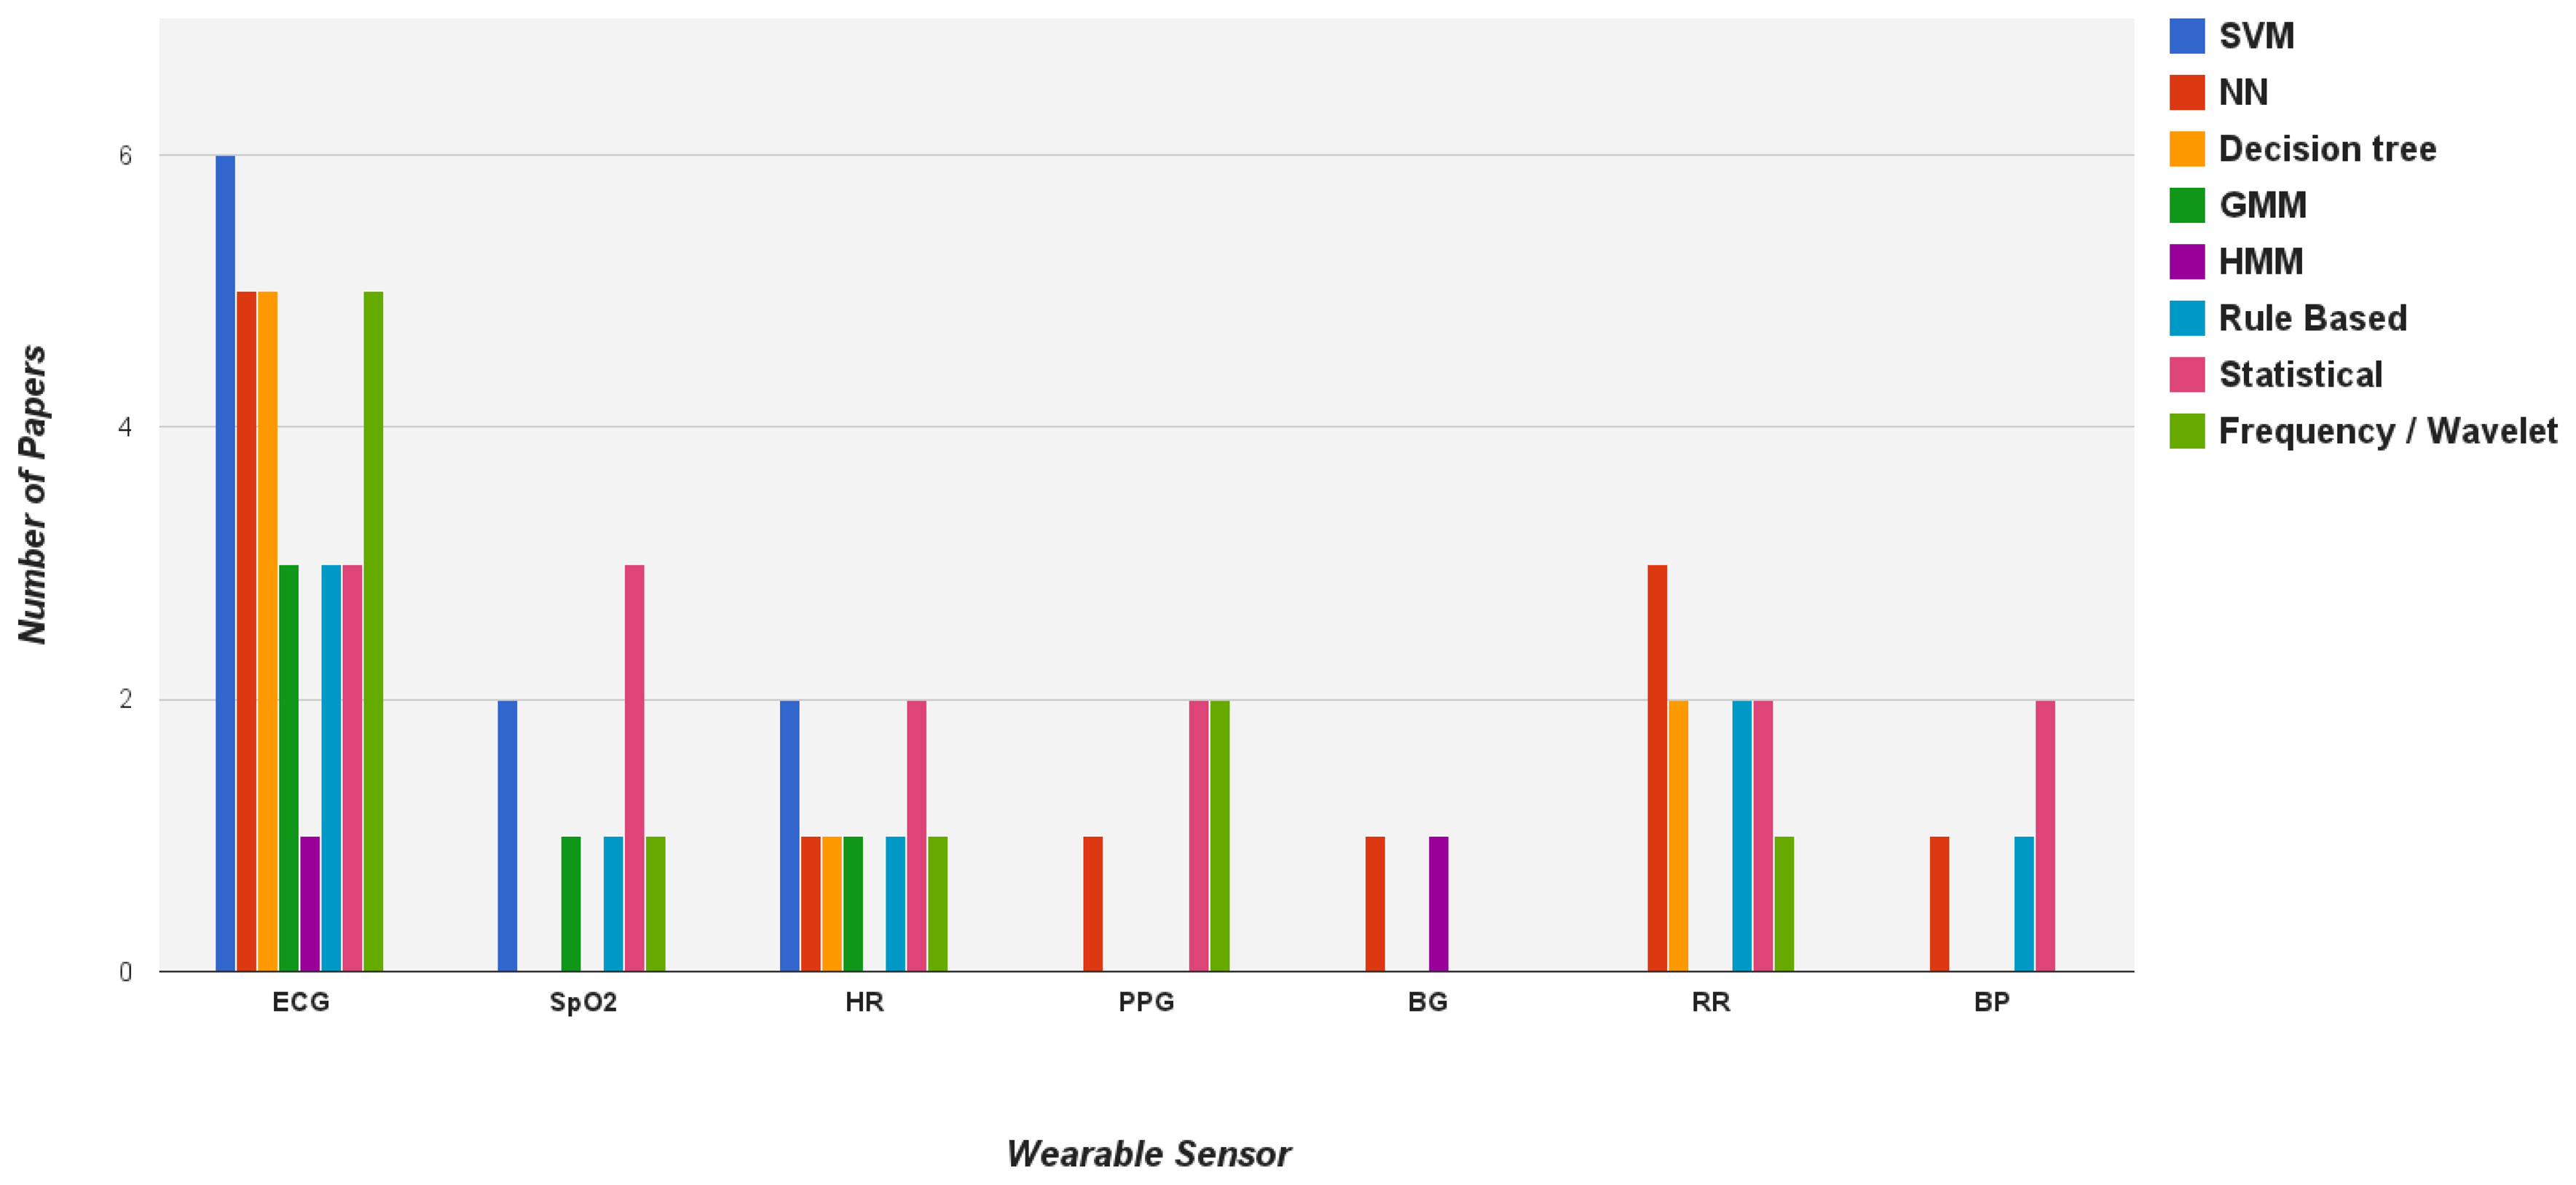
\includegraphics[width=\textwidth]{images/stateartalgorithms.png}
\caption{Comparison of some of the most common techniques used with physiological signals}
\label{fig:stateart_algorithms}
\end{figure}
